\section{Einleitung}\raggedbottom
\subsection{Motivation}
Die US-Präsidentschaftswahl 2016 gilt vielen politischen Beobachtern als eindrucksvollstes Beispiel dafür, wie von staatlicher Seite organisierte Desinformationskampagnen den politischen Diskurs nachhaltig verzerren können. Bereits zwei Jahre nach der Wahl kamen britische Wissenschaftler in Zusammenarbeit mit der Firma Graphika zu der Erkenntnis, dass ein Unternehmen mit dem Namen \glqq Internet Research Agency\grqq{}	(IRA), welches dem russischen Staat nahesteht, im großen Stil versucht hat, amerikanische Wähler via Fake-Postings in sozialen Netzwerken zu beeinflussen. In ihrem Bericht geben die Forscher an, dass mehr als 30 Millionen Benutzer im Zeitraum von 2015 bis 2017 in Berührung mit von der IRA erstellten Inhalten gekommen sind. Die Urheber jener destruktiver Inhalte werden Trolle genannt. \citep{IRAOxf18}\\
In Twitter, welches das hauptsächlich betrachtete soziale Netzwerk in dieser Arbeit sein soll, machen Trolle besonders von der Hashtag-Setzung Gebrauch. Bei einem \textit{Hashtag} handelt es sich um eine durch den Ersteller eines Beitrags vorgenommene Themenfestlegung bzw. -klassifizierung. Eine nicht durch Leerzeichen unterbrochene Zeichenkette wird durch Voranstellen eines Rautezeichens (engl. \textit{hash}) zu einem Hashtag. In der Folge kann ein \textit{Tweet} (plattformeigene Bezeichnung für einen Beitrag) durch das Benutzen der allgemeinen Suchfunktion gefunden werden. Abbildung \ref{tweetex} zeigt einen beispielhaften Tweet der IRA, welcher dem der Arbeit zugrundeliegenden Datensatz entnommen wurde und die Hashtag-Nutzung durch einen Troll illustriert.
\begin{figure}[htb]
	\begin{center}
		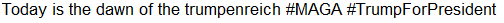
\includegraphics{bilder/Abb1.png}
		\caption{Beispiel eines IRA-Tweets}\label{tweetex}
	\end{center}
\end{figure}\\
Kommt es innerhalb eines gewissen Zeitraums zur gehäuften Benutzung eines bestimmten Hashtags, so wird dieser in den \glqq Twitter-Trends\grqq, eine Art Ranking der momentan meistgenutzten Hashtags, aufgeführt. Dies macht die Aktualität bzw. Relevanz eines gesellschaftlichen Themas direkt ablesbar. Für Trolle bietet dies aber die Möglichkeit durch geschickte zeitliche Abstimmung bestimmte Hashtags zu Trend-Hashtags zu machen und den Nutzern so aktiv die Relevanz bestimmter Themen vorzutäuschen.\\
Insgesamt sind mit den genannten Methoden verschiedenste Arten der Manipulation seitens Trollen denkbar. So können Trolle eine politische Partei oder einen Kandidaten unterstützen und versuchen, ihren Mitbewerbern zu schaden. Beispiele dafür gibt es auch in Deutschland.
So gelang es dem ultrarechten Netzwerk \glqq Reconquista Germanica\grqq{} während des TV-Duells zwischen Bundeskanzlerin Merkel und ihrem Herausforderer Martin Schulz im Jahr 2017 reichweitenstarke Tweets zu erstellen, welche Politiker diskreditieren \citep{tagesschau2020}.
Ein weitere tragende Säule von Desinformationskampagnen, welche meist in Verbindung zu Trollen steht, sind die \textit{Fake News}. Hierbei handelt es sich um Falschmeldungen bzw. Nachrichten ohne Wahrheitsgehalt, welche verbreitet werden, um die Öffentlichkeit zu manipulieren. Trolle treten hier in der Regel wechselweise als Urheber und Multiplikatoren solcher Meldungen auf.\\
Alle bisher beschriebenen Strategien sind gemeinsam als integrative Gesamtstrategie dazu geeignet, um die Ausgänge demokratischer Wahlen zu beeinflussen. Die Initiative \glqq ichbinhier e.V.\grqq{} und das Londoner \glqq Institute for Strategic Dialogue\grqq{} (ISD) kamen in einer Studie beispielsweise zu der Schlüsselerkenntnis, dass rechtsextreme Trollnetzwerke im Bundestagswahlkampf 2017 Urheber einer ausgedehnten und erfolgreichen \glqq pro-AfD-Wahlkampagne\grqq{} waren \citep{ISD18}. Das Ziel der Desinformationskampagnen, gleich ob aus dem Inland oder Ausland gesteuert, ist die Destabilisierung der demokratischen Institutionen bzw. der Demokratie als Ganzes. Aus diesem Grund möchte ich in dieser Arbeit meinen Teil dazu beitragen, dass eine Lösung für dieses Problem gefunden wird.  
\subsection{Datensätze}
Im Rahmen dieser Arbeit soll ein Verfahren entwickelt werden, welches die zuverlässige Erkennung von Troll-Inhalten auf Twitter ermöglicht. Hierbei kommen verschiedenste Techniken der Textklassifikation zum Einsatz. Diese werden auf zwei Datensätze angewandt, auf deren Eigenschaften und Ursprünge an dieser Stelle eingegangen werden soll.\\
Die Grundmenge des ersten Datensatzes ist eine von \citet{LinWar18} veröffentlichte Sammlung von rund 3 Millionen Tweets der IRA. Hier wurden die Tweets mit den zehn häufigsten Hashtags (siehe Tabelle \ref{tab_toptweets}) entnommen.\\
\begin{table}[htb]
	\begin{center}
		\begin{tabular}{|l|l||l|l|}
			\hline
			Platz & Hashtag & Platz & Hashtag \\ \hline \hline
			1	& \#news	  & 6	& \#topNews\\ 
			2	& \#sports & 7   & \#MAGA\\
			3   & \#politics & 8 & \#BlackLivesMatter\\
			4   & \#world	& 9 & \#health\\
			5	& \#local	& 10 & \#tcot\\ \hline			
		\end{tabular}
		\caption{Hashtags aus Datensatz 1}\label{tab_toptweets}
	\end{center}
\end{table}\\
Beim zweiten Datensatz handelt es sich um im Vorfeld eigens extrahierte Tweets von echten Profilen. Damit thematische Ähnlichkeit besteht wurden nur Tweets, welche die zehn Hashtags aus dem anderen Datensatz enthalten, ausgewählt. Es wurde streng darauf geachtet, dass die Datensätze disjunkt sind. Tabelle \ref{tab_datasets} zeigt zum Vergleich die wichtigsten Kennzahlen beider Datensätze.
\begin{table}[htb]
	\begin{center}
		\begin{tabular}{|l|l|l|}
			\hline
		Eigenschaft					& Troll		& Nichttroll\\ \hline \hline
		Anzahl Tweets   			& 303.036	& 324.873	\\ \hline
		unterschiedliche Autoren    & 770		& 68.706		\\ \hline
		Zeitraum					& 01/2015 - 09/2017& 01/2015 - 05/2018\\ \hline
		durchschnittliche Länge		& 78,64 Zeichen	& 122,27 Zeichen\\ \hline
		\end{tabular}
		\caption{Vergleich der Datensätze}\label{tab_datasets}
	\end{center}
\end{table}
\pagebreak